\documentclass[11pt, a4paper,spanish]{article}

\usepackage[utf8]{inputenc}
\usepackage{geometry}
\usepackage{graphicx}
\usepackage{amsmath}


\usepackage{hyperref}

\usepackage{float}

\newcommand\abs[1]{\left|#1\right|}


\title{Visualización de Datos MedioAmbientales de Castilla y León}
\author{Sergio García Prado}


\begin{document}

	\begin{titlepage}
		\centering
		{\scshape\LARGE Universidad de Valladolid \par}
		
		\vspace{1cm}
		{\scshape\Large Algoritmos y Computación\par}
		
		\vspace{1.5cm}
		{\huge\bfseries Job Shop Scheduling\par}
		
		\vspace{2cm}
		{\Large\itshape Sergio García Prado\par}

		\vfill
		Seguimiento del trabajo en: \par
		\href{https://github.com/garciparedes/Job-Shop-Scheduling-NP-Complete}{github.com/garciparedes/Job-Shop-Scheduling-NP-Complete}
		\vfill

		% Bottom of the page
		{\large \today\par}
	\end{titlepage}

	\newpage
		\tableofcontents
	\newpage
	
		\section{Introducción}
		
			\subsection{Definición del problema}
			
				\paragraph{}
				Job Shop Scheduling es un problema de optimización que se estudia en Ciencias de la Computación e Investigación de Operaciones. Ahora describiremos el problema y el objetivo que se pretende conseguir:
			
				\paragraph{}
				Supongamos que tenemos $n$ trabajos a realizar, los cuales denotamos como $J_{i}$ tal que $1 \leq i \leq n$ cada uno de distinta duración. También tenemos $r$ máquinas con las que realizar los trabajos que denotaremos por $M_{j}$ tal que $1 \leq j \leq r$. Cada una de estas es la encargada de realizar una operación concreta necesaria para finalizar cada uno de los trabajos. A cada una de estas operaciones las denotaremos por  $O_{j}{i}$ que representa la operación que se debe realizar en la máquina  $M_{j}$ del trabajo $J_{i}$ y tienen un tiempo de procesamiento de $p_{ij}$. El orden de ejecución de las operaciones en las máquinas se designa como $v_{i}$.
				\paragraph{}
				En Job Shop Scheduling el orden de las operaciones necesarias para completar el i-ésimo trabajo importa y no se puede modificar.
			 
				\paragraph{}
				El objetivo será tratar de minimizar al máximo posible el tiempo necesario para completar todas las operaciones. Para ello trataremos el problema como de decisión, es decir, buscaremos la respuesta la siguiente pregunta:  
				\newline
				{ \bf ¿Se pueden resolver los $i$ trabajos a partir de las $j$ máquinas en un tiempo menor o igual que $r$?}
				
			\subsection{Open Shop, Job Shop y Flow Shop}
			
				\paragraph{}
				Estos problemas tres problemas son muy similares entre si, ya que todos están referidos a la planificación de trabajos en más de una máquina.
				
				\begin{itemize}
				
					\item {\bf Open Shop}: El orden de realización de las operaciones {\bf no} importa.
					
					\item {\bf Job Shop}: El orden de realización de las operaciones importa.
					
					\item {\bf Flow Shop}: Cada trabajo tiene exactamente una operación por cada máquina, y todos los trabajos siguen el mismo orden de operaciones.
					
				\end{itemize}
			
			\subsection{Grafo Disyuntivo}
			
				\paragraph{}
				Una de las representaciones más claras y utilizadas para este tipo de problemas es el denominado grafo disyuntivo. Un grafo disyuntivo G = (V,C,D) contiene los siguientes elementos:
	
				\begin{itemize}
				
					\item Un conjunto V de nodos, cada uno de los cuales representa una operación, excepto dos de ellos, el nodo fuente y el nodo sumidero, que son nodos virtuales de duración 0 y representan el comienzo y el final del plan respectivamente.
					
					\item Aristas de precedencia C (conjunciones) correspondientes a las restricciones de precedencia. Son arcos dirigidos que unen operaciones correspondientes al mismo trabajo.
					
					\item Aristas de recurso D (disyunciones) correspondientes a las restricciones de re- curso. Son arcos no dirigidos que unen operaciones que se ejecutan en la misma máquina.
					
				\end{itemize}
				
				\paragraph{}
				Cada operación puede empezar cuando haya terminado la ejecución de sus operaciones predecesoras (en caso de que existan). En un grafo disyuntivo, la dirección de las flechas marca las relaciones de precedencia, de forma que si aparece una flecha dirigida de la operación p a q, esto indica que p precede a q. Es por esto que en el caso de que existan ciclos en el grafo, la solución no es válida.
				
				\begin{figure}[H]
						\centering
						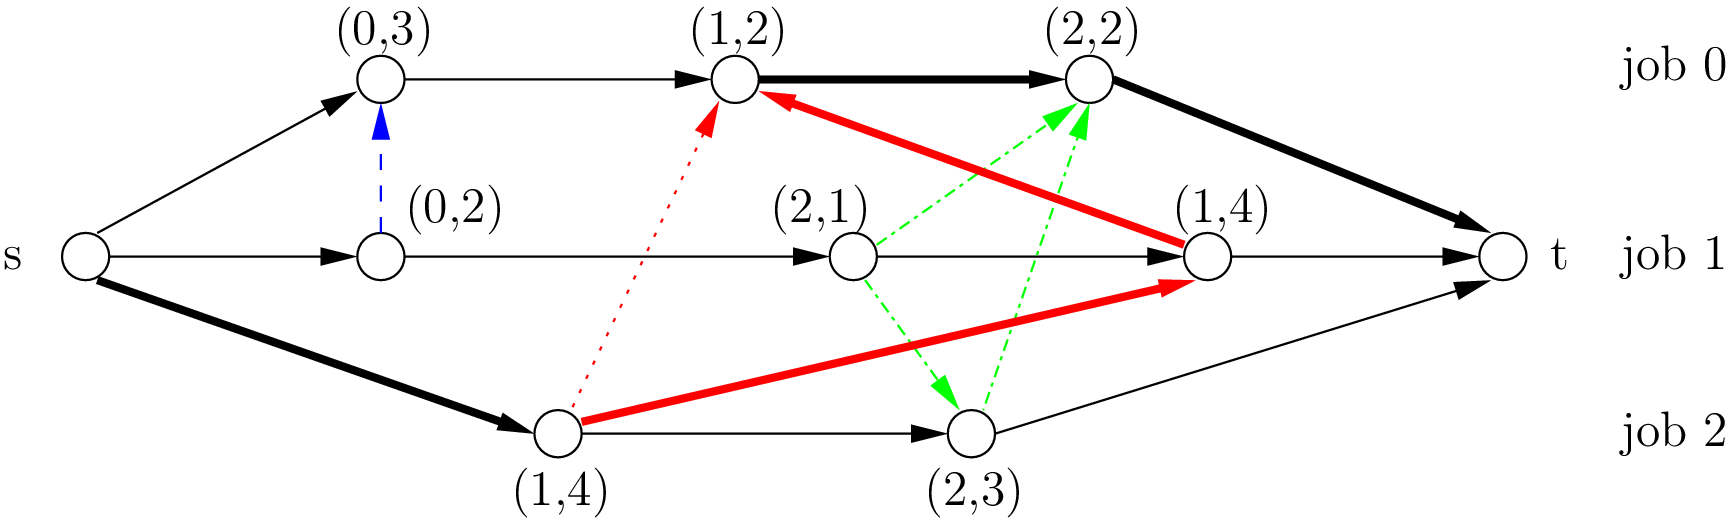
\includegraphics[width=120mm]{res/disjunctive.png}
				\end{figure}
				
			\paragraph{}
			Hoy en día Job Shop Scheduling es presentado como un problema online, lo que quiere decir que cuando le llega un nuevo trabajo, el algoritmo debe devolver una decisión antes de conocer el próximo. A pesar de que la formulación actual sea como un problema online para el análisis de reducción no se tendrá en cuenta este caso, es decir, supondremos que conocemos a priori todos los trabajos que planificar (problema offline).
		\section{Campos de Aplicación}
		
			\paragraph{}
			Los campos de aplicación de este problema son muy diversos, pero todos ellos relacionados con la organización de tareas. Encontrar la planificación óptima de un conjunto de trabajos divisibles en sub-operaciones "modularizables" en un tiempo razonable mejoraría exponencialmente la productividad. Esto aplicado al mundo empresarial reduciría muchísimo lo costes.
		
			\paragraph{}
			Un claro ejemplo de ello es la planificación de una lavandería, la cual ofrece distintos servicios como lavado, planchado, secado, arreglo de tejidos, etc. los cuales pueden ser combinados entre sí, pero deben mantener un cierto orden de realización. Los trabajos son las peticiones de los clientes, las cuales se realizan en las máquinas que hay en la lavandería. Si fuésemos capaces de encontrar la planificación de uso de las máquinas de forma óptima en un tiempo polinómico esto haría que una gran lavandería redujese tanto el tiempo como los costes de su proceso productivo.
	
		\section{Clases de Complejidad P y NP}
		
			\paragraph{}
			La relación entre las clases de complejidad P y NP es una pregunta que aún no se ha podido responder por la teoría de la complejidad computacional. En esencia, la pregunta ¿es P = NP ? significa: si es posible "verificar" rápidamente soluciones positivas a un problema del tipo SI/NO (donde "rápidamente" significa "en tiempo polinómico"), ¿es que entonces también se pueden "obtener" las respuestas rápidamente? Los recursos comúnmente estudiados en complejidad computacional son:

			\begin{itemize}
			
				\item El tiempo: mediante una aproximación al número de pasos de ejecución que un algoritmo emplea para resolver un problema.
			
				\item El espacio: mediante una aproximación a la cantidad de memoria utilizada para resolver el problema.

			\end{itemize}
			
			\paragraph{}
			Los problemas se clasifican en conjuntos o clases de complejidad (L, NL, P, PCompleto, NP, NP-Completo, NP Duro...). Nosotros nos vamos a centrar en las clases P y NP.

			\subsection{Clase P}
			
				\paragraph{}
				P es conocido por contener muchos problemas naturales, incluyendo las versiones de decisión de programa lineal, cálculo del máximo común divisor, y encontrar una correspondencia máxima. Los algoritmos de tiempo polinómico son cerrados respecto a la composición. Intuitivamente, esto quiere decir que si uno escribe una función con un determinado tiempo polinómico y consideramos que las llamadas a esa misma función son constantes y, de tiempo polinómico, entonces el algoritmo completo es de tiempo polinómico. Esto es uno de los motivos principales por los que P se considera una máquina independiente; algunos rasgos de esta máquina, como el acceso aleatorio, es que puede calcular en tiempo polinómico el tiempo polinómico del algoritmo principal reduciéndolo a una máquina más básica.
			
			\subsection{Clase NP}
				\paragraph{}
				La clase NP está compuesta por los problemas que tienen un certificado sucinto (también llamado testigo polinómico) para todas las instancias cuya respuesta es un SÍ. La única forma de que tengan un tiempo polinomial es realizando una etapa aleatoria, incluyendo el azar de alguna manera para elegir una posible solución, y entonces en etapas posteriores comprueba si esa solución es correcta. En otras palabras, dada una solución para una cierta instancia, es posible comprobar que es válida en TIME ($n^k$).


				\paragraph{Completitud de NP}
				Para analizar la pregunta P = NP, resulta muy útil el concepto de completitud NP. De manera informal, los problemas de completitud NP son los problemas más "difíciles" en NP en el sentido de que ellos son los que son más probable no se encuentren en P. Problemas NP-difíciles son aquellos para los cuales cualquier problema en NP puede ser reducido en tiempo polinómico. Los problemas de completitud NP son aquellos problemas NP-difícil que se encuentran en NP. Por ejemplo, la versión de problema de decisión del problema del viajante es completamente NP. Así ningún caso de ningún problema en NP puede ser transformado mecánicamente en una parte del problema del vendedor viajero, en tiempo polinómico. Por lo tanto, si el problema del vendedor viajero estuviera contenido en P, entonces P = NP. El problema del vendedor viajero es uno de muchos problemas NP-completos. Si cualquier problema NP-completo se encuentra contenido en P, entonces se verificaría que P = NP. Desafortunadamente, se ha demostrado que muchos problemas importantes son NP-completos y no se conoce la existencia de ningún algoritmo rápido para ellos.
				
		\section{Reducción}
		
			\paragraph{}
			Para demostrar que el problema Job Shop Scheduling pertenece a la clase NP-Complete nos basaremos en unos problemas cuya pertenencia a dicha clase ya está demostrada, por lo cual nos bastará demostrar que JobShop se puede reducir a estos. 
			
			\paragraph{}
			El método que utilizaremos será reducción polinómica, lo que quiere decir que tendremos que conseguir demostrar que existe un método de la clase P que permita transformar nuestro problema a un problema de la clase NP-Complete. Con esto se consigue que si se consiguiera demostrar que un problema de la clase NP-Complete pertenece también a la clase P, todos los problemas de la clase NP-Complete quedarían sistemáticamente demostrados como pertenecientes a la clase P por transitividad.

			\subsection{Partición}

				\paragraph{}
				{\bf Partición} es un problema NP-completo, que visto como un problema de decisión, consiste en decidir si, dado un multiconjunto (conjunto en el cual cada miembro del mismo tiene asociada una multiplicidad) de números enteros, puede éste ser particionado en dos "mitades" tal que sumando los elementos de cada una, ambas den como resultado la misma suma.
			
				\paragraph{}
				Más precisamente, dado un multiconjunto S de enteros: ¿existe alguna forma de particionar S en dos subconjuntos S1 y S2, tal que la suma de los elementos en S1 sea igual que la suma de los elementos en S2?
				
				\paragraph{}
				La solución con programación dinámica existente para resolver el problema de suma de subconjuntos, utilizando tiempo pseudo-polinómico, también es aplicable al problema de partición.
			
				\paragraph{}
				{\bf Tiempo Pseudo-Polinómico}:  un algoritmo numérico se ejecuta en tiempo pseudo-polinómico si su tiempo de ejecución es polinómico en el valor numérico de la entrada, pudiendo ser este valor exponencial en el largo de la entrada, es decir, en el número de dígitos que la conforman.  Los problemas NP-completos con algoritmos que se ejecutan en tiempo pseudo-polinómico se denominan NP-completos débiles. Un problema NP-completo se denomina NP-completo fuerte si se puede demostrar que no puede ser resuelto por algoritmos pseudo-polinómicos, salvo que se cumpla que P=NP.
			
			\subsection{3 - Partición}

				\paragraph{}
				{\bf 3-Partición} es un problema NP-completo, que consiste en decidir si dado un multiconjunto S de n = 3m enteros positivos, puede ser particionado en m subconjuntos S1, S2, …, Sm tal que la suma de sus elementos sea la misma.
			
				\paragraph{}
				Lo interesante del problema 3-Partición es que sigue siendo NP-completo incluso cuando los enteros de S están acotados por un polinomio en n. En otras palabras, el problema permanece al conjunto de problemas NP-completo incluso cuando la representación de los números en el argumento de entrada es unaria (representación mediante la repetición de un único símbolo). Es decir, el problema de la 3-partición es NP-completo en sentido estricto o estrictamente NP-completo. Esta propiedad, y en la 3-partición en general, es útil en muchas simplificaciones donde los números están representados de forma natural en unario.
	
				\paragraph{}
				Este problema fue demostrado por primera vez por Garey y Johnson mediante una solución de búsqueda 3-dimensional.
		
			\subsection{Problema de la Mochila}
				
				\paragraph{}
				El problema de la mochila es un problema de optimización combinatoria, es decir, que busca la mejor solución entre un conjunto de posibles soluciones a un problema. Modela una situación análoga al llenar una mochila, incapaz de soportar más de un peso determinado, con todo o parte de un conjunto de objetos, cada uno con un peso y valor específicos. Los objetos colocados en la mochila deben maximizar el valor total sin exceder el peso máximo. Este problema pertenece a la clase NP-Complete como demostró  Richard Karp en 1972. Enunciado matemáticamente se puede expresar como: 
				
				\paragraph{}
				Dados n enteros positivos denotados como $a_{i}$ tales que $1 < i < t$ y otro entero $b$, ¿existe un subconjunto $S \in T = \{1,...,t\} $ tal que $\sum_{i\in S}a_{i}= b$?
				
				
				
			\subsection{Job Shop}
			
				\paragraph{}
				 Ya está demostrado que los casos particulares más simples pertenecen a P con crecimiento asintótico de $O(m^2)$ para 2 trabajos y m máquinas y $O(n logn)$ para n trabajos de no más de 2 operaciones cada uno y 2 máquinas. 
				 
				\paragraph{}
				 Ahora demostraremos que este problema pertenece a la clase NP-Complete para los casos siguientes reduciéndolos al Problema de la Mochila, que ya conocemos que pertenece a la clase NP-Complete:
				 \begin{enumerate}
				  	\item n trabajos de no más de 3 operaciones cada uno en 2 máquinas
				 	\item n trabajos de no más de 2 operaciones cada uno en 3 máquinas
				 \end {enumerate}

				\paragraph{Reducción de 1:}
				
					\begin{gather}
						n = t+1 \\
						v_{i} = (M_{1}), p_{i1} = a_{i} (i \in T) \\
						v_{n} = (M_{2}, M_{1}, M_{2}), p_{n1} = b,  p_{n2} = 1,  p_{n3} = A-b \\
						y = A +1
					\end{gather}
			
					Si el problema de la mochila tiene solución, entonces existe una planificación con tiempo total de ejecución igual a $y$, como se ilustra en la figura 1. Si el Problema de la Mochila no tiene solución entonces  $\sum_{i\in S}a_{i} - b = c \neq 0$ para cada  $S \in T$, por lo que tenemos un orden de procesamiento $( \{J_{i} | i \in S\},J_{n} , \{J_{i} | i \in T-S\})$ en $M_{i}$ que:

					\begin{gather}
						c > 0 \implies  TiempoTotal \geq \sum_{i\in S}p_{i1} + p_{n2} + p_{n3} = A + c + 1 > y\\ 
						c < 0 \implies  TiempoTotal \geq  p_{n1} + p_{n2}  + \sum_{i\in T-S}p_{i1} = A - c + 1 > y
					\end{gather}
					
					Con esto se muestra que el Problema de la Mochila tiene solución solo si \textit{ n trabajos de no más de 3 operaciones cada uno en 2 máquinas} tienen solución con valor menor o igual que y.
	
					\begin{figure}[H]
						\centering
						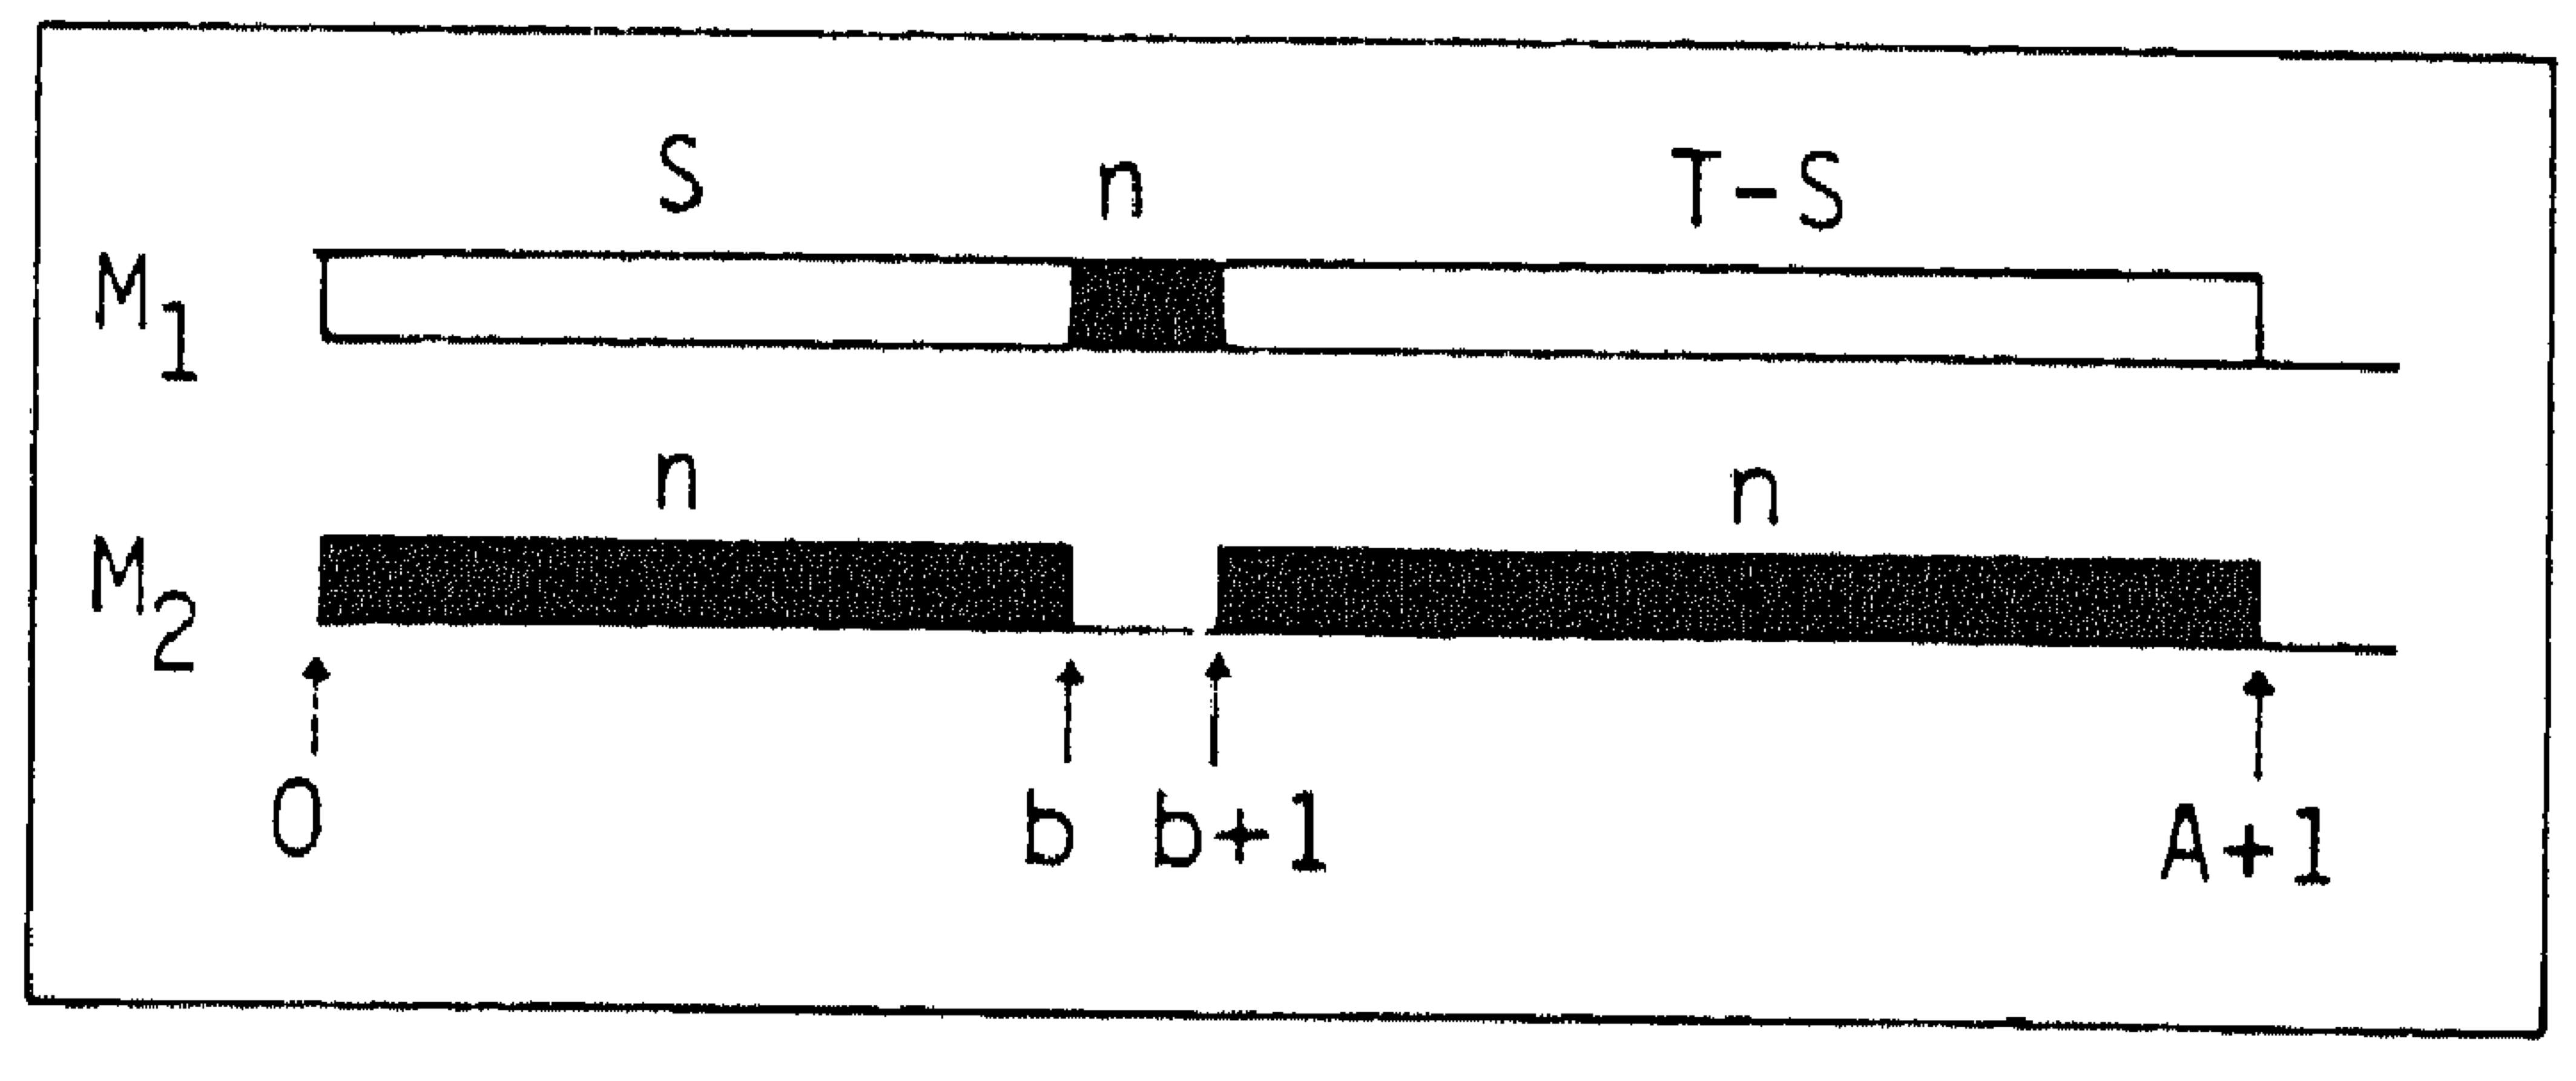
\includegraphics[width=75mm]{res/example1.png}
					\end{figure}
	
				\paragraph{Reducción de 2:}

					\begin{gather}
						n = t + 2 \\
						v_{i} = (M_{1}, M_{3}), p_{i1} = a_{i} (i \in T) \\
						v_{n-1} = (M_{2}, M_{1}), p_{n-1,1} = b,  p_{n-1,2} = 2(A-b) \\
						v_{n} = (M_{2}, M_{3}), p_{n1} = 2b,  p_{n2} = A-b \\
						y = 2A
					\end{gather}
					
					Si el problema de la mochila tiene solución, entonces existe una planificación con tiempo total de ejecución igual a $y$. Si el Problema de la Mochila no tiene solución entonces  $\sum_{i\in S}a_{i} - b = c \neq 0$ para cada  $S \in T$, por lo que tenemos un orden de procesamiento $( \{J_{i} | i \in S\},J_{n-1} , \{J_{i} | i \in T-S\})$ en $M_{i}$ que:

					\begin{gather}
						c > 0 \implies  TiempoTotal \geq \sum_{i\in S}p_{i1} + p_{n-1,1} + p_{n-1, 2} = 2A + c > y\\ 
						c < 0 \implies  TiempoTotal \geq  min\{ \sum_{i\in S}p_{i1} +p_{n-1,1}+1,p_{n1} \}+ p_{n2}  + \sum_{i\in T-S}p_{i2} = 2A + 1 > y
					\end{gather}
					
					lo que completa la prueba de equivalencia.
					
					\begin{figure}[H]
						\centering
						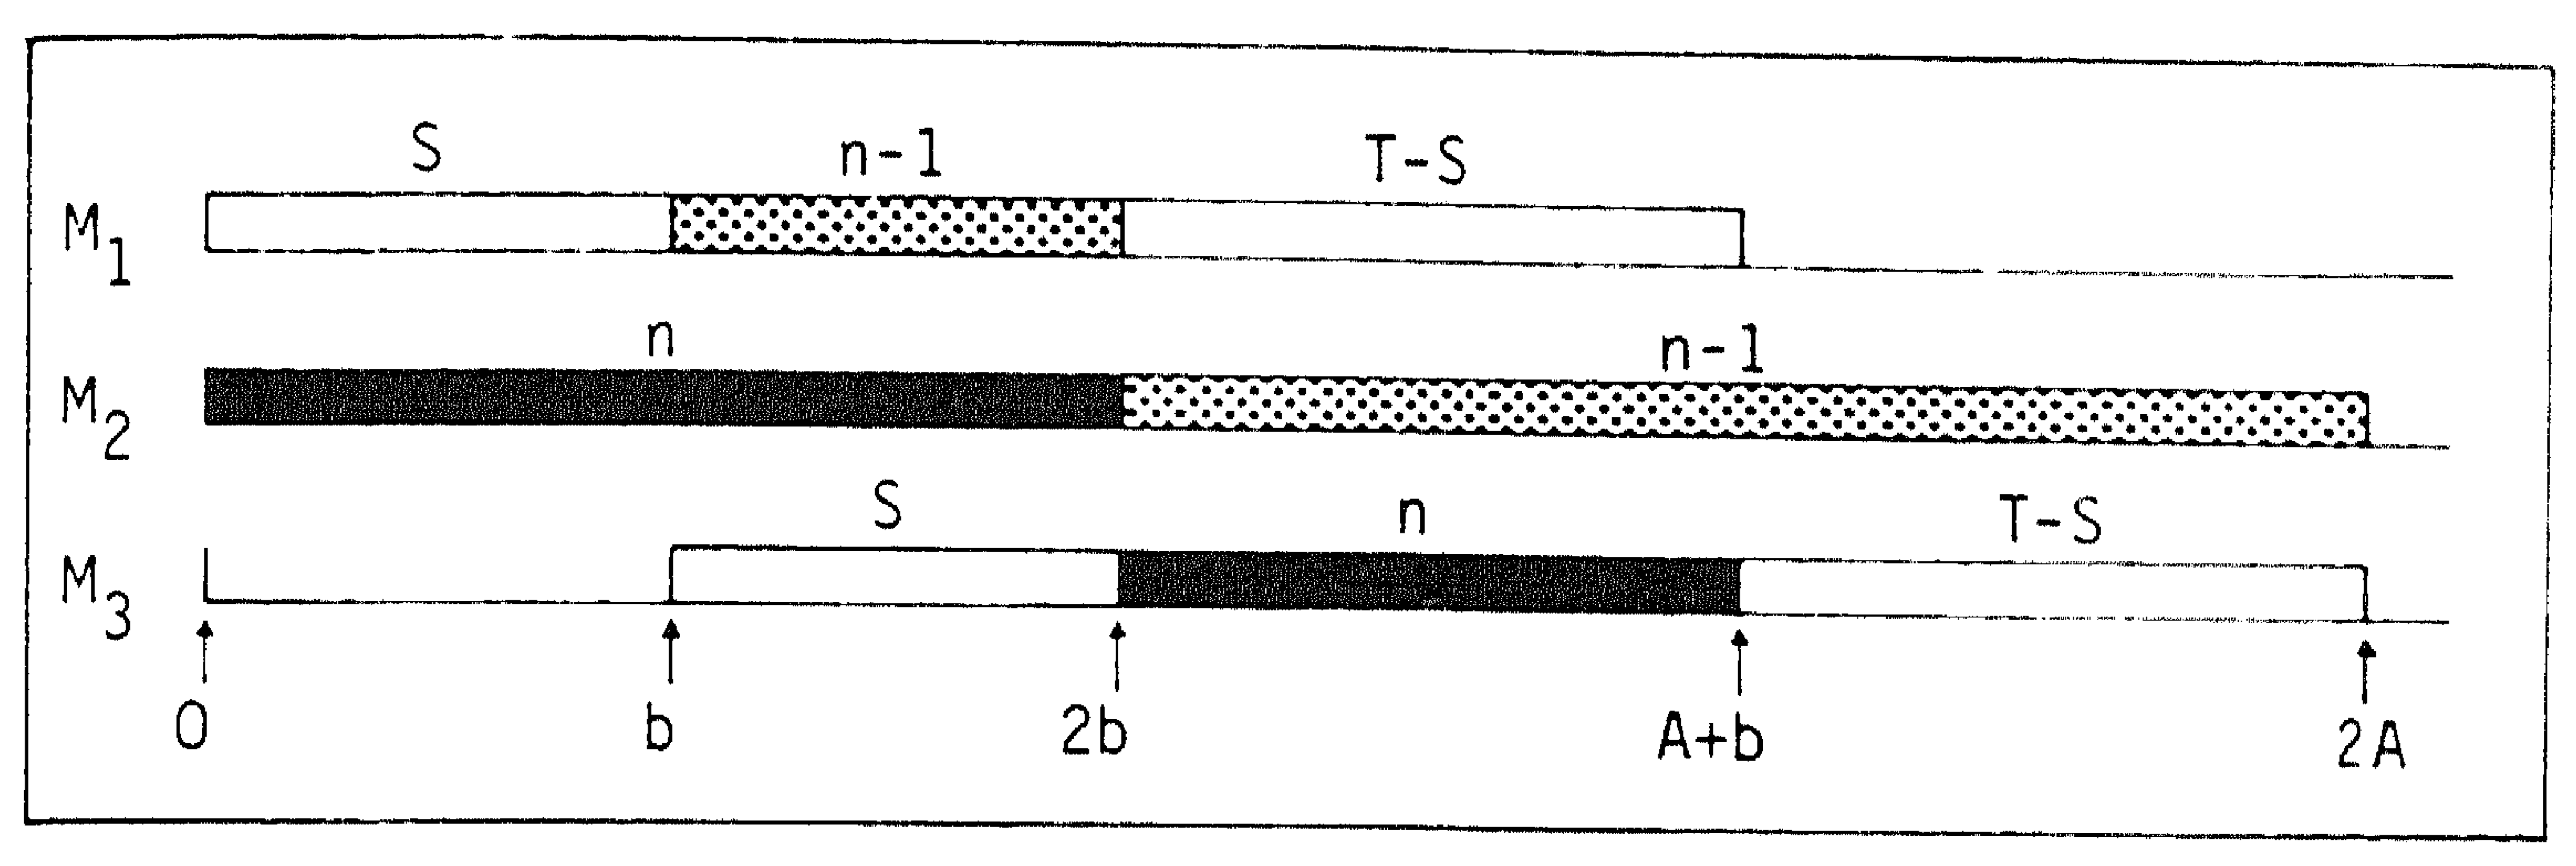
\includegraphics[width=75mm]{res/example2.png}
					\end{figure}

	\newpage

		\section{Bibliografía}

			\begin{itemize}
			
				\item \href{https://en.wikipedia.org/wiki/Job_shop_scheduling}{Wikipedia: Job Shop Scheduling}
				\item \href{http://www.rspq.org/pubs/gonz.pdf}{Operations Research: FlowShop and JobShop Schedules: Complexity and Approximation, Teofilo Gonzalez y Sartaj Sahni}
				\item \href{http://oai.cwi.nl/oai/asset/18051/18051A.pdf}{Complexity of machine scheduling problems, J. K. Lenstra, A. H. G. Rinnooy Kan, P. Brucker}
				\item \href{http://www.kecl.ntt.co.jp/as/members/yamada/galbk.pdf}{Job-shop scheduling: Takeshi Yamada, Ryohei Nakano}
				\item \href{https://en.wikipedia.org/wiki/Combinatorial_optimization}{Wikipedia: Combinatorial optimization}
				\item \href{https://en.wikipedia.org/wiki/Disjunctive_graph}{Wikipedia: Disjunctive graph}
				\item \href{https://en.wikipedia.org/wiki/Schedule_(computer_science)}{Wikipedia: Schedule}
				\item \href{https://en.wikipedia.org/wiki/P_versus_NP_problem}{Wikipedia: P versus NP problem}
				\item \href{https://www.lsi.us.es/docs/doctorado/memorias/MemoInvestigIreneBarba.pdf}{Algoritmos de planificación basados en restricciones para la sustitución de componentes defectuosos, Irene Barba Rodríguez}

			\end{itemize}


\end{document}
